\chapter{Strontium Rydberg Experiment}
\label{ch:experiment}

This chapter describes the Rydberg apparatus used in this thesis with the purpose of providing an overview of the current state of various systems for producing ultracold and quantum degenerate gases of strontium. 
Being the third ultracold strontium experiment at Rice, it was possible to leverage lessons from previous experiments, colloquially referred to as ``Neutral'' and ``Plasma'', to build quite a capable and flexible system\footnote{Collectively, the three experiments work with ultracold atomic strontium in all forms: from the ground state (Neutral) to the ions (Plasma), and everything in between (Rydberg). There is also the strontium Rydberg atomic beam experiment which produces some of }.

Although most of our system looks very similar to other ultracold strontium experiments, what makes our system uniquely suited for studying Rydberg physics is the inclusion of systems for creating, manipulating, and detecting charged particles. 
In particular, we have in-vacuum electric field plates which we can use to both cancel stray electric fields as well as to apply field ionization ramps and direct the resulting electrons (or ions) towards a microchannel plate (MCP) detector.

%Our old-school ``metal can'' setup can't compete with the optical access provided by many recently started alkaline-earth Rydberg tweezer systems using glass cells \cite{Norcia2018.PRX.8.041054, Cooper2018.PRX.8.041055, Saskin2019.PRL.122.143002}.
%There's still a place for our system which likely provides capabilities for better shielding from stray electric fields, performing SFI, and the ability to detect charged particles which, without going to significantly custom systems, are somewhat limiting on the standard glass cell setups.

\section{Producing Ultracold Gases of Strontium}

We follow the well-established laser cooling and trapping sequence for producing ultracold gases of strontium.
Detailed explanations of the various techniques and a variety of setups are available from numerous sources (e.g., \cite{Boyd2007.PhD, Mickelson2010.PhD, Martinez2012.PhD, Millen2011.PhD, Stellmer2013.PhD, Boddy2014.PhD, Barker2016.PhD, Campbell2017.PhD}) so the process will only be outlined here. 
Briefly, laser cooling and trapping of strontium gases proceeds in the following steps:
\begin{description}
	\item[Cooling and trapping on the $\nSLJ{5s^2}{1}{S}{0} \rightarrow \nSLJ{5s5p}{1}{P}{1}$ transition] \hfill \\
		The broad ${\Gamma}/{2\pi} = \SI{30.5}{\MHz}$ transition at $\SI{461}{\nm}$ is used for the first stage of cooling due its ability to scatter many photons very rapidly, exerting large forces on the atoms. 
		A ``blue'' magneto-optical trap (MOT) driving this transition typically produces samples with temperatures of about $\SIrange[range-phrase=-]{1}{2}{\milli\K}$.
		The blue MOT also loads the magnetic trap, formed by the MOT quadrupole field, with atoms in the metastable $\nSLJ{5s5p}{3}{P}{2}$ state due a small leak ($\approx \numrange[range-phrase=\colon]{1}{20000}$) of the $\nSLJ{5s5p}{1}{P}{1}$ to the $\nSLJ{5s4d}{1}{D}{2}$.
		The $\nSLJ{5s5p}{3}{P}{2}$ atoms are returned to the ground state by repumping at $\SI{481}{\nm}$
	\item[Cooling and trapping on the $\nSLJ{5s^2}{1}{S}{0} \rightarrow \nSLJ{5s5p}{3}{P}{1}$ transition] \hfill \\
		Second-stage cooling is achieved by a MOT driving the narrow ${\Gamma}/{2 \pi} = \SI{7.5}{\kHz}$ transition at $\SI{689}{\nm}$.
		Due to the narrower linewidth, the ``red'' MOT is easily able to produce samples with temperatures around $\SIrange[range-phrase=-]{1}{2}{\micro\K}$ which are suitable for loading in to optical traps.
	\item[Optical trapping and evaporative cooling] \hfill \\
		Further cooling requires optical dipole traps (ODTs) because ground-state strontium atoms have no magnetic moment and, therefore, cannot be magnetically trapped. 
		Due to the high powers required for ODTs, lasers at $\SI{532}{\nm}$ or $\SI{1064}{\nm}$ are commonly employed.
		Once cold atoms from the red MOT are loaded in to an ODT, evaporative cooling can be used to produce ultracold and quantum degenerate gases with temperatures below $\SI{1}{\micro\K}$.
\end{description}
An energy level diagram for (bosonic) strontium primarily focused on the transitions relevant for laser cooling and trapping is provided in \cref{fig:sr_level_diagram_simple}.
\begin{figure}[!htbp]
	\centering
	\includesvg[keepaspectratio, width=\textwidth, height=\textheight]{experiment/strontium_level_diagram/Sr_Energy_Level_Diagram-Boson.svg}
	\caption[]{
		\label{fig:sr_level_diagram_simple}
		A simplified level diagram of (bosonic) strontium focusing on the transitions relevant for laser cooling and trapping. 
		Solid and dashed arrows representing driven transitions and decays, respectively.}
\end{figure}

\subsection{Cooling on the $\SI{461}{\nm}$ ``Blue'' Transition}

At room temperature, strontium is a solid metal with negligible vapor pressure and thus requires an oven to sublimate strontium into a gaseous form. 
Although oven temperatures vary from setup-to-setup, they are typically around $\SIrange[range-phrase=-]{450}{750}{\celsius}$\footnote{If the setup has a nozzle heater, its temperature is generally higher than the main oven to reduce the likelihood of clogging.} \cite{Boyd2007.PhD, Ludlow2008.PhD, Schioppo2012.RSI.83.103101, Stellmer2013.PhD, Ding2016.MS, Barker2016.PhD, Campbell2017.PhD, Senaratne2018.PhD}. 
As a result, the first step in laser cooling and trapping strontium utilizes the $\SI{461}{\nm}$ $\nSLJ{5s^2}{1}{S}{0} \rightarrow \nSLJ{5s5p}{1}{P}{1}$ transition with its broad ${\Gamma}/{2 \pi} = \SI{30.5}{\MHz}$ linewidth which enables high photon scattering rates. 
\Cref{tab:blue_isotope_shift} gives the isotope shifts of the $\SI{461}{\nm}$ transitions referenced to \Sr{88}.
\begin{table}[!htbp]
	\caption[]{
		\label{tab:blue_isotope_shift}
		Isotope shifts of the $\SI{461}{\nm}$ $\nSLJ{5s^2}{1}{S}{0} \rightarrow \nSLJ{5s5p}{1}{P}{1}$ transition relative to \Sr{88}.
		Calculated from the weighted averages of values presented in \cref{tab:blue_isotope_shift_detailed,tab:hyperfine_coefficients_5s5p1P1}.
		$g$-factors for the upper state are also included.}
	\centering
	\begin{tabular}{@{}ccccc@{}}
		\toprule
		Isotope						& Lower level										& Upper level					& $\nu - \nu_{88}$ [$\si{\MHz}$]	& $g_J$ or $g_F$	\\
		\midrule	
		\Sr{88}						& $\nSLJ{5s^2}{1}{S}{0}$							& $\nSLJ{5s5p}{1}{P}{1}$		& $\num{0}$							& $\num{1}$			\\
		\midrule	
		\multirow{3}{*}{\Sr{87}}	& \multirow{3}{*}{$\nSLJf{5s^{2}}{1}{S}{0}{9/2}$}	& $\nSLJf{5s5p}{1}{P}{1}{7/2}$	& $\num{-11.3+-1.6}$				& $\num{{-2}/{9}}$	\\
									&													& $\nSLJf{5s5p}{1}{P}{1}{11/2}$	& $\num{-53.4+-1.6}$				& $\num{{2}/{11}}$	\\
									&													& $\nSLJf{5s5p}{1}{P}{1}{9/2}$	& $\num{-70.6+-1.6}$				& $\num{{4}/{99}}$	\\
		\midrule	
		\Sr{86}						& $\nSLJ{5s^2}{1}{S}{0}$							& $\nSLJ{5s5p}{1}{P}{1}$		& $\num{-124.7+-0.6}$				& $\num{1}$			\\
		\midrule	
		\Sr{84}						& $\nSLJ{5s^2}{1}{S}{0}$							& $\nSLJ{5s5p}{1}{P}{1}$		& $\num{-270.9+-0.7}$				& $\num{1}$			\\
		\bottomrule
	\end{tabular}
\end{table}

Immediately after the atoms exit the oven, they pass through a two-dimensional (2D) collimator which applies transverse optical molasses \cite{Balykin1984.JETP.63.508, Balykin1985.JOSAB.2.1776, Lett1989.JOSAB.6.2084, Joffe1993.JOSAB.10.2257, Hoogerland1996.APB.62.323} to reduce the divergence of the atomic beam.
Some experiments have incorporated a 2D magneto-optical trap (MOT) which can not only focus the atomic beam but can also deflect the atoms so that only cold atoms enter the experiment region \cite{Yang2015.EPJD.69.226}\footnote{The designs presented in \cite{Dorscher2013.RSI.84.043109, Lamporesi2013.RSI.84.063102, Nosske2017.PRA.96.053415, Nosske2018.PRA.97.039901} are probably the more ``traditional'' 2D MOT which forms a cold line of atoms that are then ``pushed'' to the main chamber.}.
In order to maximize the efficiency of the 2D collimator, elliptical beams are used to increase the intensity along the atomic beam.

Since the 2D collimator has no effect on the longitudinal velocity, they atoms are still moving at about $v_{\text{avg}} \approx \SI{500}{\meter\per\second}$\footnote{Assuming the atomic beam leaves the oven at $T = \SI{425}{\celsius}$: $v_{\text{mp}} \approx \SI{445}{\meter\per\second}$, $v_{\text{avg}} \approx \SI{483}{\meter\per\second}$, and $v_{\text{rms}} \approx \SI{514}{\meter\per\second}$ \cite{Metcalf1999.LCT}.}, much too quickly to be trapped by a MOT operating on the $\SI{461}{\nm}$ transition which has a capture velocity of about $v_C \approx \SI{14}{\meter\per\second}$\footnote{The capture velocity defined as $v_C \equiv \flatfrac{\Gamma}{k}$ where $\Gamma$ is the transition linewidth and $k$ is the transition wavevector \cite{Metcalf1999.LCT}.} \cite{Camargo2015.MS, Metcalf1999.LCT}.
The atoms are slowed longitudinally with a Zeeman slower where a spatially-varying magnetic field keeps the slowing atoms in resonance with a $\SI{461}{\nm}$ beam counterpropagating to their direction of travel \cite{Phillips1982.PRL.48.596}.
Because the  magnetic field is axial, a circularly polarized $\SI{461}{\nm}$ beam is used.
Several ideas and considerations for Zeeman slowing an atomic beam can be found in \cite{Dedman2004.RSI.75.5136, Bell2010.RSI.81.013105, Reinaudi2012.JOSAB.29.729, Hill2014.JPB.47.075006, Lebedev2014.JPB.47.155003, Krzyzewski2014.RSI.85.103104, Ohayon2015.RSI.86.103110, Hopkins2016.RSI.87.043109}.

Now that a significant portion of the atoms have been slowed by the Zeeman slower, they enter the main chamber where they are cooled and trapped by a standard six-beam $\SI{461}{\nm}$ ``blue'' MOT.
The MOT uses a quadrupole magnetic field and light detuned below atomic resonance to provide both position-dependent and velocity-dependent forces that capture and cool the atoms \cite{Raab1987.PRL.59.2631, Metcalf1999.LCT, Foot2005.Atomic}. 
Blue MOTs typically produce samples of atoms around $\SIrange[range-phrase=-]{1}{2}{\milli\kelvin}$.
Some experiments (e.g., \cite{Barker2016.PhD}) implement a ``cold blue MOT'' stage where the detuning, intensity, and quadrupole gradient are ramped to obtain colder temperatures for improved transfer efficiency to the red MOT but we found that our temperatures are sufficient for decent transfer.

\begin{figure}[!htbp]
	\centering
	\includesvg[keepaspectratio, width=\textwidth, height=\textheight]{experiment/blue_system/old_blue_MOT.svg}
	\caption[]{
		\label{fig:old_blue_MOT}
		A picture of the \Sr{88} blue MOT taken on 2014/08/29 through one of the $\SI{2.75}{\inch}$ viewports.
		The strontium oven and Zeeman slower are located off to the right.
		With the electric field plates separated by about $\SI{1}{\inch}$, this blue MOT likely has a diameter of close to $\SI{0.5}{\inch}$.}
\end{figure}

Although the $\SI{461}{\nm}$ light is capable of scattering many photons per second, the Doppler limit of this transition is about $T_{D} = \SI{732}{\micro\kelvin}$\footnote{For the $\SI{461}{\nm}$ transition: $k_{B} T_{D} \equiv \flatfrac{\hbar \Gamma}{2} = \SI{732}{\micro\kelvin}$, $k_{B} T_{r} \equiv \flatfrac{\hbar^2 k^2}{2 M} = \SI{512}{\nano\kelvin}$.} \cite{Metcalf1999.LCT}.
Although sub-Doppler cooling is not available in the bosonic isotopes due to the lack of hyperfine structure, it has been observed in \Sr{87} where the blue MOT temperature was measured to be about $\SI{300}{\micro\kelvin}$ \cite{Xu2003.PRL.90.193002, Xu2003.JOSAB.20.968}.
Interestingly, as noted in \cite{Xu2003.PRL.90.193002}, cooling bosonic alkaline-earth atoms on the $\SLJ{1}{S}{0} \rightarrow \SLJ{1}{P}{1}$ transition typically yields temperatures a few times the Doppler cooling limit \cite{Kisters1994.APB.59.89, Xu2002.PRA.66.011401, Xu2003.JOSAB.20.968}.

\subsection{Magnetic Trap and Repumping}

The $\nSLJ{5s^2}{1}{S}{0} \rightarrow \nSLJ{5s5p}{1}{P}{1}$ transition is not completely closed where $\nSLJ{5s5p}{1}{P}{1}$ atoms can leak to the $\nSLJ{5s4d}{1}{D}{2}$ state. 
The branching ratio for this decay path was found to be ${A\pqty{\SLJ{1}{P}{1} \rightarrow \SLJ{1}{S}{0}}}/{A\pqty{\SLJ{1}{P}{1} \rightarrow \SLJ{1}{D}{2}}} \approx \num{20E3}$ \cite{Cooper2018.PRX.8.041055}\footnote{Previous measurements suggested that this branching ratio was about $\numrange[range-phrase=\colon]{1}{50000}$ \cite{Hunter1986.PRL.56.823}}.
About $\num{2/3}$ of the $\nSLJ{5s4d}{1}{D}{2}$ atoms then decay to the $\nSLJ{5s5p}{3}{P}{1}$ which subsequently decays to the $\nSLJ{5s^2}{1}{S}{0}$ and return to the $\SI{461}{\nm}$ cooling cycle.
The remaining ${1}/{3}$ decay to the long-lived metastable $\nSLJ{5s5p}{3}{P}{2}$ state with a lifetime of about $\SI{520}{\second}$ \cite{Yasuda2004.PRL.92.153004}, effectively removing them from the blue MOT cooling cycle.
Of the $\nSLJ{5s5p}{3}{P}{2}$ states, the low-field seeking $m_J = 1, 2$ states can become trapped in the quadrupole magnetic field of the blue MOT \cite{Loftus2002.PRA.66.013411, Nagel2003.PRA.67.011401}.
This decay path, initially seen as a loss from the blue MOT, ends up being a powerful tool for accumulating atoms in a 	metastable reservoir at roughly the same temperature as the blue MOT and was an essential tool in overcoming the $\SI{\approx 0.5}{\percent}$ natural abundance of \Sr{84} to produce the first strontium BECs \cite{Stellmer2009.PRL.103.200401, Martinez2009.PRL.103.200402}.

The magnetic trap is also crucial for laser cooling and trapping multiples isotopes. 
As seen in \cref{tab:blue_isotope_shift}, the isotope shifts are comparable to the linewidth meaning a blue MOT can only efficiently trap a single isotope at a time. 
The key to trapping multiple isotopes is to utilize the automatic accumulation of $\SLJ{3}{P}{2}$ atoms, which are dark to the $\SI{461}{\nm}$ cooling light, in the magnetic trap.
Multiple isotopes can be loaded in to the magnetic trap by simply operating a blue MOT tuned for a particular isotope and then tuning the laser to trap another isotope. 
This sequential loading typically starts with the most abundant isotope, since those atoms will spend the most time the magnetic trap, before tuning the $\SI{461}{\nm}$ to cool and trap subsequent isotopes. 
Loading rates into the magnetic trap could be improved by implementing a ``depumping'' laser that pumps atoms from the $\nSLJ{5s5p}{3}{P}{1}$ state to the $\nSLJ{5s5p}{3}{P}{2}$ \cite{Barker2015.PRA.92.043418}.

Before moving on to the next cooling stage, atoms in the metastable reservoir need to be returned to the ground state.
Several transitions have been explored for repumping atoms out of the metastable reservoir, each of which has varying advantages and disadvantages \cite{Courtillot2005.EPJD.33.161, Boyd2007.PhD, Ludlow2008.PhD, Barker2015.PRA.92.043418, Campbell2017.PhD, Cooper2018.PRX.8.041055, Mickelson2009.JPB.42.235001, Stellmer2013.PhD, Stellmer2014.PRA.90.022512, Moriya2018.JPC.2.125008, Mason2013.BS, Stellmer2014.PRA.90.022512, Moriya2018.JPC.2.125008, Wongwaitayakornkul2013.BS, Camargo2015.MS, Ding2016.MS, Couturier2018.RSI.89.043103, Hu2019.PRA.99.033422}\footnote{An excellent overview of the various repumping transitions is presented in \cite{Stellmer2013.PhD}.}.
On our experiment, we drive the $\nSLJ{5s5p}{3}{P}{2} \rightarrow \nSLJ{5p^2}{3}{P}{2}$ transition at $\SI{481}{\nm}$.
One of the key advantages of this transition is that the upper state is $\SLJ{3}{P}{2}$ so it only requires a single laser to clear out the magnetic trap since the $\nSLJ{5p^2}{3}{P}{2}$ can only decay to either the $\nSLJ{5s5p}{3}{P}{1}$ or $\nSLJ{5s5p}{3}{P}{2}$ states. 
Another advantage of this transition is that the hyperfine structure in \Sr{87} of the doubly-excited $\nSLJ{5p^2}{3}{P}{2}$ state is expected to be small meaning the hyperfine shifts should be predominantly due to the $\nSLJ{5s5p}{3}{P}{2}$ state which are known \cite{Heider1977.PRA.16.1371, Onishchenko2019.PRA.99.052503}. 
\begin{figure}[!htbp]
	\centering
	\includegraphics[keepaspectratio, width=\textwidth, height=\textheight]{experiment/repumper_system/20180327-preliminary_84Sr_87Sr_repumper_spectra/repumper_spectra.pdf}
	\caption[]{
		\label{fig:repumper_spectra}
		Representative number of \Sr{84} and \Sr{87} atoms returned to the $\nSLJ{5s^2}{1}{S}{0}$ ground state from the magnetic trap varying the $\SI{481}{\nm}$  laser frequency.
		The labeled arrows indicate the expected relative hyperfine energy shifts of the various $\nSLJF{5s5p}{3}{P}{2}{F}$ states in \Sr{87} calculated using only the hyperfine $A$ and $B$ constants of the $\nSLJ{5s5p}{3}{P}{2}$ state from \cite{Heider1977.PRA.16.1371}.}
\end{figure}
As seen in \cref{fig:repumper_spectra}, the $A = \SI{-212.765(1)}{\MHz}$ and $B = \SI{67.215(15)}{\MHz}$ hyperfine constants of the $\nSLJ{5s5p}{3}{P}{2}$ state \cite{Heider1977.PRA.16.1371} captures the observed energy splittings in the $\nSLJF{5s5p}{3}{P}{2}{F} \rightarrow \nSLJ{5p^2}{3}{P}{2}$ transitions quite well.
When multiple isotopes are loaded into the magnetic trap, it will be necessary to apply the appropriate frequency shifts to the repump laser so that all isotopes are recovered efficiently. 

Other uses for the magnetically trapped metastable strontium could be for magnetic transport of atoms from a ``collection'' chamber to a ``science'' chamber.
It should also be mentioned that the magnetic trap is not always necessary nor preferred depending on the particular isotope and experiment being performed. 
Keeping a repumper on can result in higher initial blue MOT loading rates by preventing accumulation of atoms in the metastable reservoir which can drastically reduce cycle times. 
This approach may be of interest for experiments looking to have fast cycle times such as in optical tweezer experiments working with \Sr{88} \cite{Cooper2018.PRX.8.041055, Norcia2018.PRX.8.041054, Hanley2018.PhD, Jackson2019.arXiv.1904.03233}.
An interesting idea is mentioned in \cite{Bowden2019.arXiv.1907.13429} where atoms in the magnetic trap are laser cooled using the $\nSLJ{5s5p}{3}{P}{2} \rightarrow \nSLJ{5s4d}{3}{D}{3}$ transition at $\SI{2.92}{\um}$ before being returned to the $\nSLJ{5s^2}{1}{S}{0}$ state for loading in to an optical lattice.

\subsection{Cooling on the $\SI{689}{\nm}$ ``Red'' Transition}

After the $\SI{461}{\nm}$ cooling stage, the strontium atoms are typically around $\SIrange[range-phrase=-]{1}{2}{\milli\kelvin}$ whereas efficient loading of atoms in to optical dipole traps require sample temperatures closer to $\SIrange[range-phrase=-]{1}{2}{\milli\kelvin}$.
A ``red'' MOT operating on the narrow $\nSLJ{5s^2}{1}{S}{0} \rightarrow \nSLJ{5s5p}{3}{P}{1}$ transition at $\SI{689}{\nm}$ bridges this gap. 
With $\Gamma/2\pi = \SI{7.5}{\kHz}$, the Doppler limit $T_{D} \approx \SI{180}{\nano\kelvin}$ is comparable to the recoil limit of $T_{r} \approx \SI{230}{\nano\kelvin}$.
\begin{table}[!htbp]
	\caption[]{
		\label{tab:red_isotope_shift}
		Isotope shifts of the $\SI{689}{\nm}$ $\nSLJ{5s^2}{1}{S}{0} \rightarrow \nSLJ{5s5p}{3}{P}{1}$ transition, relative to \Sr{88}.
		Calculated from the weighted averages of the values in \cref{tab:red_isotope_shift_detailed}.
		$g$-factors for the upper state are also included.}
	\centering
	\begin{tabular}{@{}ccccc@{}}
		\toprule
		Isotope						& Lower level										& Upper level					& $\nu - \nu_{88}$ [$\si{\MHz}$]	& $g_J$ or $g_F$	\\
		\midrule	
		\Sr{88}						& $\nSLJ{5s^2}{1}{S}{0}$							& $\nSLJ{5s5p}{3}{P}{1}$		& $\num{0}$							& $\num{{3}/{2}}$	\\
		\midrule	
		\multirow{3}{*}{\Sr{87}}	& \multirow{3}{*}{$\nSLJf{5s^{2}}{1}{S}{0}{9/2}$}	& $\nSLJf{5s5p}{3}{P}{1}{7/2}$	& $\num{1351.937+-0.027}$			& $\num{{-1}/{3}}$	\\
									&													& $\nSLJf{5s5p}{3}{P}{1}{9/2}$	& $\num{221.689+-0.013}$			& $\num{{2}/{33}}$	\\
									&													& $\nSLJf{5s5p}{3}{P}{1}{11/2}$	& $\num{-1241.465+-0.018}$			& $\num{{3}/{11}}$	\\
		\midrule	
		\Sr{86}						& $\nSLJ{5s^2}{1}{S}{0}$							& $\nSLJ{5s5p}{3}{P}{1}$		& $\num{-163.81443+-0.00026}$		& $\num{{3}/{2}}$	\\
		\midrule	
		\Sr{84}						& $\nSLJ{5s^2}{1}{S}{0}$							& $\nSLJ{5s5p}{3}{P}{1}$		& $\num{-351.59+-0.11}$				& $\num{{3}/{2}}$	\\
		\bottomrule
	\end{tabular}
\end{table}
Following \cite{Loftus2004.PRA.70.063413}, MOTs can be characterized by the ratio of the transition linewidth ($\Gamma$) to the single photon recoil frequency shift ($\omega_R$) with typical MOTs operating in the regime $\flatfrac{\Gamma}{\omega_R} \gg 1$ compared to narrow line MOTs where $\flatfrac{\Gamma}{\omega_R} \sim 1$.
Operating in the $\flatfrac{\Gamma}{\omega_R} \sim 1$ regime where a few photon recoils can kick an atom out of resonance with the cooling lasers leads to very different dynamics.
The differences in dynamics are especially apparent in the shape of the bosonic red MOTs \cite{Stellmer2013.PhD, Stellmer2014.arXiv.1307.0601}.
The fermionic red MOT may look similar to a $\flatfrac{\Gamma}{\omega_R} \gg 1$ MOT but it's shape is due to complications arising from hyperfine structure.
An excellent description of how the narrow $\SI{689}{\nm}$ ``red'' MOT works for both the bosons and fermion is presented in \cite{Stellmer2013.PhD}\footnote{The ``Red MOT Bible''.} with additional resources in \cite{Boyd2007.PhD, Stellmer2014.arXiv.1307.0601}.

Considering first the bosonic case, the ${\Gamma}/{2\pi} = \SI{7.5}{\kHz}$ transition is a bit too narrow to effectively capture the $\SI{\sim 2}{\milli\kelvin}$ atoms from the blue MOT.
In order to increase the transfer efficiency, the spectrum of the red MOT light is artificially broadened by frequency modulation, typically by a few megahertz, which enables addressing of multiple velocity classes of atoms from the blue MOT.
Once enough atoms have been captured in the ``broadband'' red MOT, the frequency modulation and intensity are ramped down\footnote{Reducing the frequency modulation essentially increases the intensity of each comb tooth in the FM spectrum.} to a narrow or single-frequency red MOT which increases the sample density and reduces the temperature.

While the bosonic isotopes of strontium behave like an ideal $J=0 \rightarrow J=1$ MOT as described in texts (e.g., \cite{Metcalf1999.LCT, Foot2005.Atomic}) and it is relatively straightforward to produce samples below $\SI{2}{\micro\kelvin}$, the hyperfine structure of \Sr{87} poses a challenge.
Since the ground state has (essentially) no magnetic moment, the position-dependent Zeeman shift is only experienced by the $\SLJ{3}{P}{1}$ state with a $g_{F} m_{F}$-dependent magnitude.
This results in both a restoring force for some positions and transitions and an anti-trapping force for other transitions and positions.
Narrow line laser cooling of \Sr{87} was first achieved by the Tokyo group through the use of a ``trap'' laser resonant with the $\nSLJf{5s^2}{1}{S}{0}{9/2} \rightarrow \nSLJf{5s5p}{3}{P}{1}{11/2}$ transition and a second ``stir'' laser resonant with $\nSLJf{5s^2}{1}{S}{0}{9/2} \rightarrow \nSLJf{5s5p}{3}{P}{1}{9/2}$ to quickly redistribute the population and take advantage of the Clebsch-Gordan coefficients so that, on-average, the atoms experience a trapping force \cite{Mukaiyama2003.PRL.90.113002, Stellmer2013.PhD}.

Due to the large isotope shifts compared to the ${\Gamma}/{2\pi} = \SI{7.5}{\kHz}$ linewidth of the transition (see \cref{tab:red_isotope_shift}), red MOTs for multiple isotopes can be operated simultaneously.
This ability compliments the metastable reservoir exceedingly well since, when switching from the blue MOT to the red MOT, the magnetic field gradient is lowered from about $\SIrange[range-phrase=-]{30}{70}{\gauss\per\cm}$ to about $\SIrange[range-phrase=-]{1}{10}{\gauss\per\cm}$ which releases the atoms from the magnetic trap. 
It is during the switching time that the repump light is applied so all the isotopes released from the metastable reservoir are returned to the $\nSLJ{5s^2}{1}{S}{0}$ ground state, ready for the red MOT to capture and cool. 
After laser cooling on the \SI{689}{\nm} transition, our sample temperatures are typically $\SIrange[range-phrase=-]{1}{2}{\micro\kelvin}$, which is sufficient for loading into an optical dipole trap (ODT).

An alternative method to the broadband red MOT is saw-tooth wave adiabatic passage (SWAP) cooling which eschews the traditional broadband red MOT in favor of carefully designed frequency ramps that adiabatically transfer atoms between the $\SLJ{1}{S}{0}$ and $\SLJ{3}{P}{1}$ states \cite{Norcia2018.PhD, Norcia2018.NJP.20.023021, Bartolotta2018.PRA.98.023404, Muniz2018.arXiv.1806.00838}.
The advantage of this method is particularly apparent for \Sr{87} which eliminates the need for the ``stir'' laser. 
The drawback is that the temperatures achieved seem to be limited to about $\SI{10}{\micro\kelvin}$ due to the need to maintain efficient adiabatic transfer \cite{Norcia2018.PhD}.
A promising technique is to use SWAP cooling instead of the broadband red MOT to capture atoms from the blue MOT before transferring to a single-frequency red MOT to reach colder temperatures \cite{Snigirev2019.PRA.99.063421}.

\subsection{Optical Dipole Trap (ODT)}

Strontium in the $\nSLJ{5s^2}{1}{S}{0}$ ground state has no magnetic moment meaning it cannot be magnetically trapped \footnote{There is interest in producing quantum degenerate gases of alkaline-earth atoms in metastable states \cite{Barker2016.PRA.93.053417}, some of which are magnetically trappable. Quantum degenerate gases of metastable atoms have been realized for helium \cite{Robert2001.Science.292.461, Santos2001.PRL.86.3459, McNamara2006.PRL.97.080404}.} and requires the use of optical dipole traps (ODTs) and evaporative cooling to attain temperatures below $\SI{1}{\micro\kelvin}$.
Optical dipole traps work by using intense, off-resonant light to shift atomic energy levels. 
Since the amount of shift a state experiences is dependent on the intensity, an intensity gradient leads to spatially-varying force such that, when appropriately designed, will attract atoms to the area of highest, or lowest, intensity. 
For a two-state atom with ground state $\ket{g}$ and excited state $\ket{e}$ separated by energy $\hbar \omega_0$ and coupled by a laser with frequency $\omega$, the AC Stark shift can be written as (e.g., see \cite{Grimm1999.arXiv.9902072, Steck.QuantumAtomOptics})
\begin{equation}
	\label{eq:odt_potential}
	{\Delta}E\pqty{\va{r}}	=	-\frac{3 \pi c^2}{2 \omega_0} \pqty{\frac{\Gamma}{\omega_0 - \omega} + \frac{\Gamma}{\omega_0 + \omega}} I\pqty{\va{r}}
					=	-\frac{1}{2 \epsilon_0 c} \Re\bqty{\alpha\pqty{\omega}} I\pqty{\va{r}}
\end{equation}
Oftentimes, the details of the transition are collected in to a complex frequency-dependent ``polarizability'' $\alpha\pqty{\omega}$. 
A quick and easy way to generalize \cref{eq:odt_potential} to a multilevel atom is to treat the multiple levels as individual two-level subsystems and then sum the contributions due to off-resonant coupling in each two-level subsystem (e.g., \cite{Katori1999.JPSJ.68.2479, Ye2008.Science.320.1734}). 
An accurate calculation of the AC Stark shift would require diagonalizing the Hamiltonian which includes all the states in the atom.

% Strontium in the $\nSLJ{5s^2}{1}{S}{0}$ ground state has no magnetic moment meaning it cannot be magnetically trapped\footnote{There is some interest in producing quantum degenerate gases of alkaline-earth atoms in metastable states some of which are magnetically trappable (e.g., the $\nSLJ{5s5p}{3}{P}{2}$) \cite{Barker2016.PRA.93.053417}. Quantum degenerate gases of metastable atoms have been realized for helium \cite{Robert2001.Science.292.461, Santos2001.PRL.86.3459, McNamara2006.PRL.97.080404}.} and requires the use of optical dipole traps (ODTs) to perform evaporation.
% **** Work through details of this derivation! ****
% Following the derivation in \cite{Ludlow2008.PhD, Steck.QuantumAtomOptics} with more details in \cref{app:odt_derivation}, we start by considering a two-level atom with states $\ket{g}$ and $\ket{e}$ separated by energy $\hbar \omega_{0}$.
% Applying an off-resonant laser with frequency $\omega_{L}$ field couples these two states which shifts their energy levels by 
% \begin{equation}
	% \label{eq:ac_pol}
	% \Delta E	= -\frac{E^{2}_{0}}{4} \qty(\frac{2 \abs{d}^{2}}{\hbar} \frac{\omega_{0}}{\omega_{0}^{2} - \omega_{L}^{2}})
				% = -\frac{E^{2}_{0}}{4} \alpha\qty(\omega_{L})
% \end{equation}
% where  $\alpha\qty(\omega_{L})$ is the (dipole) polarizability and $d \equiv \mel{g}{\va{d}}{e}$ is the dipole matrix element.
% A simple generalization to a multi-level atom is relatively straightforward by summing the contributions for other levels.
% The resulting  polarizability can be written as
% \begin{equation}
	% \alpha_{g}\qty(\omega_{L})	= \frac{2}{\hbar} \sum_{e} \abs{d_{ge}}^{2} \frac{\omega_{ge}}{\omega_{ge}^{2} - \omega_{L}^{2}}
% \end{equation}
% Here, $g$ doesn't necessarily need to be the ground state.
% Spatial confinement is achieved by considering $I = \flatfrac{c \epsilon_{0} E_{0}^{2}}{2}$ so by designing a spatially-varying intensity $I\qty(\va{r})$.
% *** FIX EQUATION ***
% \begin{equation}
	% \label{eq:U_odt}
	% \alpha_{g}\qty(\omega_{L})	= \frac{2}{\hbar} \sum_{e} \abs{d_{ge}}^{2} \frac{\omega_{ge}}{\omega_{ge}^{2} - \omega_{L}^{2}}
% \end{equation}
% *** FIX EQUATION ***

For strontium, the red MOT spatial distribution and the particular isotope(s) being loaded needs to be taken in to account when designing an ODT.
While the fermionic red MOT traps atoms in an ellipsoidal volume around the MOT quadrupole center (where $\abs*{B} = 0$), the atoms in a bosonic red MOT tend to form a thin shell below the quadrupole center \cite{Stellmer2013.PRA.87.013611, Stellmer2014.arXiv.1307.0601}. 
As a result, improved loading of atoms into an ODT can be obtained by ``mode-matching'' the trapping volume of the ODT to better match the spatial distribution of atoms in the red MOT.
The preferred ODT geometry appears to be a high-aspect ratio horizontal ``pancake'' or ``light sheet'' where the tight axis is along gravity as this matches well with the shape of the bosonic red MOT \cite{Stellmer2013.PRA.87.013611, Stellmer2013.PhD, Barker2016.PhD, Oppong2015.MS, Campbell2017.PhD}. 
%Our main trap is currently a single ``sheet'' beam with waist sizes of about ** $\SI{26}{\um} \times \SI{260}{\um}$ **\footnote{Some traps used by other groups: $\SI{18}{\um} \times \SI{250}{\um}$ \cite{Stellmer2013.PRA.87.013611}; $\SI{22.8}{\um} \times \SI{228}{\um}$ and $\SI{16}{\um} \times \SI{270}{\um}$ \cite{Barker2016.PhD, Reschovsky2017.PhD}; $\SI{17}{\um} \times \SI{340}{\um}$ \cite{Oppong2015.MS, Campbell2017.PhD}.}

The specific isotope(s) being worked with also have an effect on both loading into an ODT as well as on their evaporation due to their wildly varying intra- and inter-isotope scattering lengths (see \cref{tab:sr_scattering_lengths_long}). 
\begin{table}[!htbp]
	\caption[]{
		\label{tab:sr_scattering_lengths_long}
		Measured $s$-wave scattering lengths ($a_s$) of strontium given in [$\si{\bohr}$].}
	\centering
	\begin{tabular}{@{}cccc@{}}
		\toprule
		Isotope				& $a_s$ \cite{Martinez2008.PRA.78.062708}	& $a_s$ \cite{Stein2010.EPJD.57.171}	& $a_s$ \cite{Aman2018.PRA.98.053441}		\\
		\midrule
		{\Sr{88}-\Sr{88}}	& \num{-1.4(6)}								& \num{-2.00(27)}						& 											\\
		{\Sr{87}-\Sr{87}}	& \num{96.2(1)}								& \num{96.198(68)}						& 											\\
		{\Sr{86}-\Sr{86}}	& \num{823(24)}								& \num{798(12)}							& \num[parse-numbers=false]{810.6(3)(9)}	\\
		{\Sr{84}-\Sr{84}}	& \num{122.7(3)}							& \num{122.762(92)}						& 											\\
		{\Sr{88}-\Sr{87}}	& \num{55.0(2)}								& \num{54.819(92)}						& 											\\
		{\Sr{88}-\Sr{86}}	& \num{97.4(1)}								& \num{97.374(69)}						& 											\\
		{\Sr{88}-\Sr{84}}	& \num{1790(130)}							& \num{1658(54)}						& 											\\
		{\Sr{87}-\Sr{86}}	& \num{162.5+-0.5}							& \num{162.25(21)}						& 											\\
		{\Sr{87}-\Sr{84}}	& \num{-56(1)}								& \num{-57.61(61)}						& 											\\
		{\Sr{86}-\Sr{84}}	& \num{31.9(3)}								& \num{31.65(14)}						& 											\\
		\bottomrule
	\end{tabular}
\end{table}
The first strontium BECs were achieved with \Sr{84}, which has a convenient $a_s = \SI{123}{\bohr}$ scattering length \cite{Stein2010.EPJD.57.171}, was easily evaporated to quantum degeneracy in low aspect ratio traps \cite{Martinez2009.PRL.103.200402, Stellmer2009.PRL.103.200401}.
An unpolarized degenerate Fermi gas of \Sr{87} was also obtained in a nearly-circular ODT \cite{DeSalvo2010.PRL.105.030402} but spin-polarized degenerate Fermi gases requires sympathetic cooling and thus requires trapping multiple isotopes \cite{Stellmer2013.PRA.87.013611}.
Early work towards producing quantum degenerate gases of \Sr{88} and \Sr{86} were hindered by the tight waists of the ODT beams which leads to inelastic losses of \Sr{86} \cite{Poli2005.PRA.71.061403, Ferrari2006.PRA.73.023408}. 
It was only by going to a large-volume high-aspect-ratio ODT was a BEC of \Sr{86} realized \cite{Stellmer2010.82.041602}.
The first BEC of \Sr{88} was achieved by sympathetic cooling with (unpolarized) \Sr{87} in a nearly spherical trap \cite{Mickelson2010.PRA.81.051601}.

Some recent work towards developing systems for trapping strontium in optical tweezer arrays showed results that an ODT around $\SIrange[range-phrase=-]{501}{520}{\nm}$ is close to a ``magic'' wavelength\footnote{A wavelength is ``magic'' when two (or more) states experience the same shift such that there is no differential shift between them \cite{Ye2008.Science.320.1734, Ludlow2015.RMP.87.637}.} for the $\nSLJ{5s^2}{1}{S}{0} \rightarrow \nSLJ{5s5p}{3}{P}{1}$ transition \cite{Norcia2018.PRX.8.041054, Cooper2018.PRX.8.041055}.
It should be noted that both our current $\SI{1064}{\nm}$ ODT and a ``green'' ODT are both expected to be repulsive for strontium Rydberg states \cite{Mukherjee2011.JPB.44.184010, Topcu2016.JPB.49.144004}.

\section{Vacuum System}

An overview of our vacuum system is shown in \cref{fig:vacuum_system} with the some of the primary components labeled.
\begin{figure}[!htbp]
	\centering
	\includesvg[keepaspectratio, width=\textwidth, height=\textheight]{experiment/vacuum/rydberg_vacuum_system.svg}
	\caption[]{
		\label{fig:vacuum_system}
		Overview of the strontium Rydberg apparatus highlighting the main sections of the vacuum system and various components.}
\end{figure}
Perhaps the most noticeable aspect of our vacuum system is that it was designed to have the majority of the horizontal laser beams about $\SI{3.5}{\inch}=\SI{8.89}{\cm}$ from the surface of the optical table.
Keeping the beams at this height eliminated the need for rigid supporting structures to elevate the entire vacuum system along with the associated need for raised optical platforms for getting beams to the vacuum chamber. 

To facilitate vertically propagating beams, two holes were cut through the table with a semicircle at the end of the table for the vertical 2D collimator arm and a $\SI{10}{\inch}$ diameter circle under the main chamber for MOT and dipole trap beams.
We had originally planned on mounting vertical optics directly to the main chamber but decided instead to mount them to a single elevated platform above the main chamber and another platform on the underside of the table. 
Adding the breadboard under the table required tapping threads on the underside of the table.
The major disadvantage of our current setup is the long distance between the undertable breadboard and the bottom of the main chamber, about $\SI{12}{\inch}$\footnote{The thickness of the optical table.}, which makes it difficult to design, install, and align sensitive vertical beams.

\subsection{Source-side Vacuum System}
\label{ssec:source-side_vacuum}

This section of the vacuum chamber is where the strontium oven and 2D collimator are located and produces the atomic beam of strontium for cooling and trapping.
Although there are various designs for strontium ovens \cite{Senaratne2015.RSI.86.023105, Schioppo2012.RSI.83.103101}, and even commercial systems, we used a simple design that has shown success on the older strontium experiments in the laboratory.
The design is simple with a single Watlow FIREROD cartridge heater\footnote{These are neat little devices which come with leads for both the resistive heating element and an integrated thermocouple.} providing the majority of the heating power to the oven.
An array of capillary tubes forms a nozzle to provide some degree of collimation and resistive heater wire is wrapped around them to reduce the effects of strontium building up in the capillary tubes and clogging.
We typically run our main FIREROD oven heater around $\SI{425}{\celsius}$ with the nozzle heater around $\SI{390}{\celsius}$\footnote{Ideally, the nozzle should be hotter than the reservoir to reduce the likelihood of clogging the capillary tubes but it's likely that our actual oven temperature is a bit lower due to the FIREROD thermocouple sensor being buried in the cartridge heater body rather than at the location of the strontium.}.
\Cref{fig:neutral_sr_oven} shows a recently fabricated strontium oven made to replace the one on the Neutral apparatus and is very similar to the one on our setup with the major difference being that it is mounted on the smaller $\SI{2.75}{\inch}$ flange whereas ours is mounted on a $\SI{3.375}{\inch}$ flange. 
\begin{figure}[!htbp]
	\centering
	\includesvg[keepaspectratio, width=\textwidth, height=3in]{experiment/atomic_oven/neutral_sr_oven.svg}
	\caption[]{
		\label{fig:neutral_sr_oven}
		Neutral's new strontium oven during construction before the nozzle thermocouple and heating wires were attached. 
		The design is very similar to our oven but is mounted on a $\SI{2.75}{\inch}$ flange instead of a $\SI{3.375}{\inch}$ flange.
		(Left) Oven without heat shield.
		(Right) After adding heat shield.}
\end{figure}
The larger flange provides some extra room for various feedthroughs without being too cramped.

Immediately after the atoms exit the oven, they pass through the two-dimensional (2D) collimator stage which applies transverse optical molasses to increase the flux of atoms down the Zeeman slower. 
To maximize the limited amount $\SI{461}{\nm}$ laser power, the beams are elliptical to maximize the intensity on the atoms and a single beam is recycled through the four arms of the 2D collimator.
The long arms also help to prevent strontium buildup on the AR coated viewports.
\begin{figure}[!htbp]
	\centering
	\includesvg[keepaspectratio, width=\textwidth, height=\textheight]{experiment/atomic_oven/atomic_beam.svg}
	\caption[]{
		\label{fig:atomic_beam}
		(Left) Cross-section image of the source-side vacuum system. 
		(Right) Picture of the fluorescing atomic beam as viewed down the vertical arm of the two-dimensional (2D) collimator.
		A reflection of the atomic beam off the vertical retro mirror is also visible.}
\end{figure}

Before the atoms leave this section of the vacuum system and enter the Zeeman slower, they pass through a differential pumping tube\footnote{A cylinder of OFHC (oxygen-free high thermal conductivity) copper with a coaxial through hole with approximate dimensions of $\diameter = \SI{0.3}{\inch}$ by $L = \SI{2.4650}{\inch}$.} with a conductance $C \approx \SI{0.85}{\liter\per\second}$ which helps maintain the pressure differential between the source and experiment sides of the system. 
The pressure in the source side is typically higher than the experiment side and is around $\SI{7.6E-9}{\Torr}$\footnote{MiniVac ion pump controller outputting $\SI{7.9}{\mV}=\SI{7.9E-6}{\A}$ for the  rebuilt VacIon Plus 75 Starcell on 2019/06/13.}.
We suspect the ion pump on the source side is being restricted by the zero-length reducer which adapts the $\SI{4.5}{\inch}$ flange on the source-side vacuum chamber to the $\SI{6}{\inch}$ flange on the Varian ion pump.

A shutter and a gate valve was also installed between the source-side vacuum system and the Zeeman slower. 
The shutter allows us to physically block the atomic beam which should extend the time between needing to change the Zeeman slower entrance window. 
The gate valve should, in principle, allow us to isolate the source-side vacuum system from the rest of the chamber to facilitate reloading the strontium oven without venting the entire vacuum chamber but we found this valve to be somewhat leaky when we initially pumped out our system\footnote{Something similar was noticed by the Weld group at UCSB and they used two gate valves to separate their atomic source from their UHV main chamber \cite{Senaratne2018.PhD}.}.

\subsection{Zeeman Slower}

Since an oven is required to produce enough strontium vapor for trapping, a Zeeman slower is needed to slow the atoms down so that they can be captured by the MOT. 
Our Zeeman slower is detailed in \cite{Camargo2015.MS} so it will only be briefly covered here. 
The Zeeman slower uses a spatially-varying axial magnetic field and circularly-polarized light to keep the atoms resonant with a light propagating counter to the direction of the atomic beam so that they continuously scatter photons as they slow \cite{Phillips1982.PRL.48.596}.
Our particular design is a ``spin-flip''-type slower where the amplitude of the axial magnetic field crosses zero between the ends.
The Zeeman slower coil was constructed in multiple layers to allow tailoring of the resulting field to match the desired profile.
Each layer was attached to the Zeeman slower with thermally-conductive epoxy\footnote{Emerson and Cuming STYCAST 2762 or STYCAST 2762 FT with Catalyst 14, 17, or 17M-1.} and the resulting magnetic field measured before wrapping the next layer.
Due to the relatively long Zeeman slower\footnote{The inner wall of the Zeeman slower is about $\diameter = \SI{0.6940}{\inch}$ by $L = \SI{18.8296}{\inch}$.} ($C \approx \SI{1.4}{\liter\per\second}$), it's conductance should be reduced, helping to maintain differential pumping between the source and experiment sides.

For cooling, the Zeeman slower was custom made with a double wall that acts as a water cooling jacket.
The inner wall separates the cooling water from UHV.
The magnetic field coils are wrapped around the outer wall.
Due to space constraints, the source-side is welded to a $\SI{2.75}{\inch}$ flange whereas it's connected to the main chamber by a $\SI{2.125}{\inch}$ flange.
These flanges are also where cooling water enters and exits the jacket.
It's possible to avoid water-cooling by using a permanent magnet Zeeman slower \cite{Lebedev2014.JPB.47.155003, Cheiney2011.RSI.82.063115, Reinaudi2012.JOSAB.29.729, Hill2014.JPB.47.075006} but the magnetic field would likely require significant shielding and/or more demanding cancellation efforts in order for it to not interfere with other aspects of the experiment. 

\subsection{Experiment-side Vacuum System}

The experiment-side vacuum system can be broken down in to the main chamber where experiments take place and a ``pumping tower'' which provides a high-conductance path to the vacuum pumps.
The custom main chamber \footnote{Fabricated by Huntington Mechanical Labs.} features:
\begin{itemize}
	\item Recessed top and bottom flanges which bring the $\SI{2.75}{\inch}$ viewports closer to the center of the chamber while providing room for the MOT coils to fit around the viewport.
	The in-vacuum electric field plates are mounted to the bottom flange which has eleven $\SI{10}{\kV}$ safe high voltage (SHV) feedthroughs.
	\item Six (6) $\SI{2.75}{\inch}$ horizontal viewports provide optical access for the various trapping (e.g., MOT and ODT) beams and the imaging system.
	\item Three (3) $\SI{1.33}{\inch}$ horizontal viewports used for the various $\SI{689}{\nm}$ and $\SI{320}{\nm}$ excitation beams.
	These are oriented perpendicular and parallel to the MCP, allowing us to apply bias magnetic fields along the MCP axis to reduce electron deflection by the Lorentz force.
	\item Room for a Photonis miniTOF micro-channel plate (MCP) detector.
	\item A conical expansion to a $\SI{6}{\inch}$ flange for increased conductance to the vacuum pumps.
\end{itemize}
Most of the viewports were anti-reflection (AR) coated for $\SI{461}{\nm}$, $\SI{689}{\nm}$, and $\SI{1064}{\nm}$ with the transmission shown in \cref{fig:viewport_ar-coating}.
\begin{figure}[!htbp]
	\centering
	\includegraphics[keepaspectratio, width=\textwidth, height=\textheight]{experiment/vacuum/reynard_corporation-ar_coating/viewport_ar-coating.pdf}
	\caption[]{
		\label{fig:viewport_ar-coating}
		Transmission data of the Reynard Corporation\protect\footnotemark anti-reflection (AR) coating on the $\SI{1.33}{\inch}$ and $\SI{2.75}{\inch}$ viewports from MDC Vacuum Products.
		It's fortuitous that the AR coating should be very good for $\SI{698}{\nm}$ (clock transition) and reasonable for $\SI{532}{\nm}$ and $\SI{813}{\nm}$ should we ever decide to use traps at those wavelengths.}
\end{figure}
\footnotetext{I would like to thank Robyn Miller at Reynard Corporation for finding and sending me the reflection and transmission data from the order we placed six years ago.}
Vacuum pressure on the experiment-side is maintained by a $\SI{75}{\liter\per\second}$ ion pump\footnote{Gamma Vacuum TiTan 75S-CVX-6S-SC-N-N.} located at the top of the pumping tower.
The ion pump current suggests the vacuum on this side is at about $\SI{3.4E-9}{\Torr}$\footnote{MiniVac ion pump controller outputting $\SI{-4.8}{\mV}=\SI{4.8E-6}{\A}$ for the Gamma Vacuum TiTan 75S on 2019/06/13.}.
Additional pumping is provided by a non-evaporable getter (NEG)\footnote{SAES CapaciTorr D 200.} located about halfway up the pumping tower. 
In retrospect, we should have also included a titanium sublimation pump (TSP) for additional pumping capability.

Since we do not have a 2D deflection MOT, strontium from the atomic beam will deposit on the Zeeman slower entrance viewport overtime\footnote{Neutral has tried using Plasma's pulsed Nd:YAG laser to perform ablation on their coated Zeeman viewport with a moderate level of success.}.
A $\SI{3.375}{\inch}$ gate valve separates the Zeeman slower viewport from the main chamber and facilitates changing this viewport once it gets coated with strontium.

\section{Magnetic Field Trim Coils}

Three pairs of Helmholtz coils are used to cancel stray magnetic fields and to apply a bias field.
The $X$-axis and $Y$-axis coil pairs produce fields in the horizontal plane parallel to the table surface and are oriented such that the $X$-axis produce a field towards or away from the MCP whereas the $Y$-axis produces a field perpendicular to this axis.
The $Z$-axis coils produces a field along the vertical axis perpendicular to the surface of the table.

Both the horizontal ($X$-axis and $Y$-axis) trim coils are constructed from {$\num{17.5}$ AWG} wire\footnote{MWS Wire Industries 17.5 HAPT-200 (NEMA MW 35-C).} with \num{45} turns wound on aluminum U-channel and held together with polyimide tape.
Due to the choice of keeping the center of the chamber at $\SI{3.5}{\inch}$ above the table surface, this required the horizontal ($X$-axis and $Y$-axis) trim coils to be centered at this height leading to their rectangular geometry instead of square or circular.
\begin{figure}[!htbp]
	\centering
	\includesvg[keepaspectratio, width=\textwidth, height=\textheight]{experiment/trim_coils/trim_coils.svg}
	\caption[]{
		\label{fig:trim_coils}
		Magnetic field trim coils around main chamber for nulling stray fields and/or applying bias fields.
		The trim coil axes are defined relative to the MCP (equivalently, the $\SI{1.33}{\inch}$ viewports for the Rydberg excitation lasers) and gravity with the $X$-axis (blue) oriented towards the MCP, the $Z$-axis (red) pointing upwards perpendicular to the table surface, and the $Y$-axis (green) perpendicular to the $X$ and $Z$ axes (following the right-hand rule, of course).}
\end{figure}

The vertical ($Z$-axis) coils were wound on circular aluminum U-channel forms and fit around the outside of the top and bottom flanges of the main chamber which allowed us to put many turns on them. 
The circular U-channels used as the forms also feature a radial slice, filled with epoxy, to mitigate the generation of eddy currents. 
In retrospect, we should made the horizontal coils beefier (especially along the $X$-axis) in order generate larger bias fields along the MCP axis and increase detection efficiency. 
We found that having bias fields along other directions (i.e., not towards/away from the MCP) reduced our detection efficiency, likely due to the Lorentz force steering electrons away from the MCP. 

\section{Dual MOT Coils}
\label{sec:dual_mot_coils}

One of the things we did differently from the previous strontium experiments is that we have two pairs of MOT coils instead of a single pair where the larger pair is used for the blue MOT while the smaller pair for the red MOT (see \cref{fig:dual_mot_coils}).
This allows us to use two different current drivers without needing a single supply that has the dynamic range to provide the $\SI{\sim 40}{\ampere}$ to generate the $\SI{\sim 40}{\gauss\per\cm}$ gradient for the blue MOT while also generating a low-noise $\SI{\sim 1}{\gauss\per\cm}$ gradient for the red MOT.
\begin{figure}[!htbp]
	\centering
	\includesvg[keepaspectratio, width=\textwidth, height=\textheight]{experiment/mot_coils/dual_mot_coils.svg}
	\caption[]{
		\label{fig:dual_mot_coils}
		(Left) Picture of our assembled dual MOT coils on a test setup. 
		(Right) CAD rendering of how they are centered around the windows of the recessed flanges on the main chamber.}
\end{figure}
A drawing of the dual MOT coils can be found in \cref{ap:dual_MOT_coils}.

The blue MOT coils are constructed from square tubular wire\footnote{S{\&}W Wire 125SQ DPG/BARE (NEMA 46-C).} which is hollow inside for cooling water and produce a magnetic field gradient of about $\SI{1.25}{\gauss\per\cm\per\ampere}$ along the tight axis.
The coils are typically run with around $\SIrange[range-phrase=-]{40}{50}{\ampere}$ from a power supply\footnote{TDA-Lambda Genesys 8-90-IS510-U which can supply up to $\SI{8}{\volt}$ and $\SI{90}{\ampere}$.} set for fixed-current output.
A power MOSFET\footnote{An IXYS IXFN 340N07.} is used for quickly turning the current on and off.
%We so far haven't included a flyback diode although the MOSFET we use seems to include an internal flyback diode.
%These coils produce a magnetic field gradient of about $\SI{1.25}{\gauss\per\cm\per\ampere}$.

The red MOT coils are constructed from square {$\num{13}$ AWG} copper wire\footnote{MWS Wire Industries 13 SQ HML-240 (NEMA MW 20-C).} and are epoxied to the undersides of the blue MOT coils, placing them closer to the center of the vacuum chamber. 
A homebuilt voltage-controlled current driver\footnote{Powered by an APEX PA12(A) power operational amplifier.} provides the current but we should be able to use any current driver capable of supplying up to about $\SI{5}{\ampere}$. 
The red MOT coils produce a magnetic field gradient of about $\SI{1}{\gauss\per\cm\per\ampere}$.

\begin{figure}[!htbp]
	\centering
	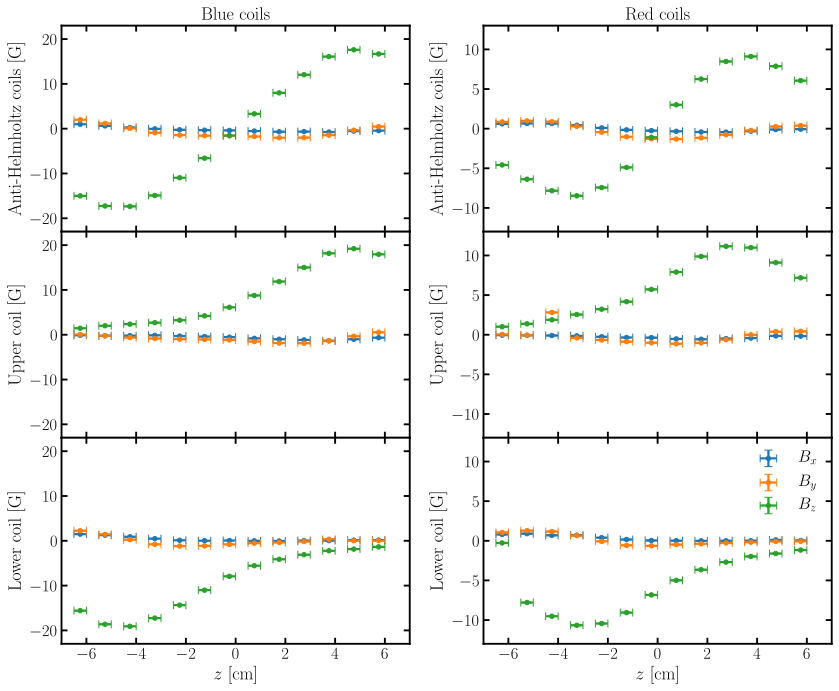
\includegraphics[keepaspectratio, width=\textwidth, height=\textheight]{experiment/mot_coils/mot_coil_fields.pdf}
	\caption[]{
		\label{fig:dual_mot_coil_fields}
		Blue MOT coil (left) and red MOT coil (right) magnetic fields measured along the $z$-axis on the test setup shown in \cref{fig:dual_mot_coils} with $I = \SI{4}{\ampere}$.
		The uncertainties are estimated to be $\pm \SI{2.5}{\cm}$ and $\pm \SI{0.05}{\gauss}$.
		The non-zero measured values of $B_x$ and $B_y$ suggest that the probe was slight off the $z$-axis.
		There also appears to be a slight systematic shift in the zero-crossing of the anti-Helmholtz coils likely due to an uncertainty in determining the physical center of the coils.}
\end{figure}

% **
% It would have been nice to have an extra MOSFET switch on the blue MOT coils so that we'd be able to apply extremely large fields along the Z-axis such as e.g. Pedro's experiment Feshbach coils.
% We're not too worried about not having this capability since ground-state strontium has no magnetic Feshbach resonances and the fact that we've observed a decrease MCP detection efficiencly we believe is due to the Lorentz force as the MCP is oriented along the X-axis.
% **

\section{Laser Systems for Producing Cold and Ultracold Strontium Gases}

\Cref{fig:trapping_beams} gives an overview of the orientation of our various laser cooling and trapping beams.
\begin{sidewaysfigure}[!htbp]
	\centering
	\includesvg[keepaspectratio, width=\paperwidth, height=\paperheight]{experiment/laser_beams/trapping_beams.svg}
	\caption[]{
		\label{fig:trapping_beams}
		Cross-section of the vacuum system (viewed from above) and a simplified diagram of the various laser beams.}
\end{sidewaysfigure}

\subsection{$\SI{461}{\nm}$ ``Blue'' Laser System}

The experiment currently has three blue diode lasers in a master-slave configuration that provides all the $\SI{461}{\nm}$ power for our experiment.
In a master-slave setup, a single (typically low-power) ``master'' external cavity diode laser (ECDL) is frequency stabilized relative to the atomic transition and is used to injection lock higher-power ``slave'' lasers to increase the available laser power \cite{Shimada2013.RSI.84.063101, Hosoya2015.RSI.86.073110}.
The master laser is locked relative to the $\nSLJ{5s^2}{1}{S}{0} \rightarrow \nSLJ{5s5p}{1}{P}{1}$ transition in a homebuilt strontium cell using Doppler-free saturated absorption spectroscopy.
The error signal is obtained by modulating the axial magnetic field in the saturated absorption cell and using circularly-polarized pump and probe beams.
Some details about our blue cooling system can be found in \cite{Camargo2015.MS, Ding2016.MS}.

Our current ECDL master laser\footnote{New Focus TLB-6802: a Littman-Metcalf external cavity diode laser (ECDL).} outputs about $\SI{40}{\mW}$.
Although this laser tunes well and generally remains single-mode when tuning between the various isotopes, we have been very disappointed with output mode quality which appears to be a Hermite-Gaussian {TEM\tsub{00}} as seen in \cref{fig:VP-0024_output}.
\begin{figure}[!htbp]
	\centering
	\includegraphics[keepaspectratio, width=\textwidth, height=\textheight]{experiment/blue_system/VP-0024/VP-0024_output.png}
	\caption[]{\label{fig:VP-0024_output}
		Output beam profile from the New Focus VP-0024 $\SI{461}{\nm}$ master laser.
		Although this image was taken after we received the laser back from repair, it exhibits a similar output mode as when we first received the laser.}
\end{figure}
Due to this poor output mode, a D-mirror was used to split the beam into two nearly-Gaussian beams, each of which was directed to a slave laser for injection locking. 
After using the laser for about six years, the piezo tuning element died and the laser had to be sent back for repairs.
While the laser was undergoing repairs, the injection locking setup was modified so that the two slave lasers are injection locked from the output of a single-mode polarization maintaining (SMPM) fiber so that we can easily change master lasers should this laser die again.
We also noticed some weird grounding and noise issues with the New Focus laser system which seemed very sensitive to the particular cables connecting the feedback circuit to the laser driver\footnote{Similar grounding and noise issues with the New Focus laser was mentioned by Sara Campbell in Jun Ye's group. She documents their experiences in \cite{Campbell2017.PhD}.}.
We also have concerns about the long-term cost-effectiveness and reliability of the New Focus ECDL\footnote{During the piezo repair, New Focus recommended installation of a new diode and the initially quoted cost, for both the repair and new diode, was about half of buying a new ECDL system. This was significantly reduced after extended discussions with the company.} and have purchased a Toptica $\SI{461}{\nm}$ ECDL system\footnote{The Toptica $\SI{461}{\nm}$ laser is capable of outputting about $\SI{100}{\mW}$.} as a future replacement and to enable additional experiments. 

\begin{sidewaysfigure}[!htbp]
	\centering
	\includesvg[keepaspectratio, width=\paperwidth, height=\paperheight]{experiment/blue_system/blue_system.svg}
	\caption[]{
		\label{fig:blue_system}
		Simplified diagram of the $\SI{461}{\nm}$ laser system in the opaque enclosure.}
\end{sidewaysfigure}

Light from the master laser currently injection locks two slave lasers for boosting the available $\SI{461}{\nm}$ power for the experiment.
We have previously tried homebuilding our own $\SI{461}{\nm}$ slave laser with a can-opened blue diode\footnote{Nichia NDB4216E - a non-AR coated diode with about $\SI{100}{\mW}$ of output power.} but found it to be unsatisfactory. 
We ended up going with two New Focus TLB-6802-IJ\footnote{From what we can tell, these are simply their standard TLB-6802 without the grating and probably using the Nichia NDB4216E non-AR coated diode which is specified to output about $\SI{100}{\mW}$.} both of which output about $\SI{100}{\mW}$ of power.
The ``MOT'' slave is injection locked at the same frequency as the master laser and its power is split between the blue MOT, 2D collimator, and the imaging beam.
The injection beam for the ``Zeeman'' slave is first shifted by $\SI{-535}{\MHz}$ relative to the master laser before injection locking the laser. This allows all the power out from the slave to be used for operating the Zeeman slower instead of taking a hit in power going through an AOM.

The entire $\SI{461}{\nm}$ system is located at the opposite end of our table from the vacuum system and is boxed in an opaque enclosure to contain the blue light, even a little of which can lead to heating our samples. 
Mechanical shutters\footnote{Hard drive shutters are used as we've found them to be the most reliable.} are used to provide $\SI{100}{\percent}$ extinction.

\subsection{$\SI{481}{\nm}$ Repumping System}

Before moving on to the narrow line red MOT, the atoms in the metastable reservoir are dark to both the $\SI{461}{\nm}$ and the $\SI{689}{\nm}$ cooling light and must be brought back to the ground state.
The current $\SI{481}{\nm}$ repumper system is shown in \cref{fig:repumper_system} with light provided by a Toptica DL 100\footnote{The laser is equipped with a {LD-0488-0060-1} diode.} which outputs about $\SI{14}{\mW}$ of power that is shared between the Rydberg, Neutral, and Plasma experiments.
\begin{figure}[!htbp]
	\centering
	\includesvg[keepaspectratio, width=\textwidth, height=\textheight]{experiment/repumper_system/repumper_system.svg}
	\caption[]{
		\label{fig:repumper_system}
		Simplified diagram of our current $\SI{481}{\nm}$ repumper laser system.
		A portion of the light form the $\SI{481}{\nm}$ external cavity diode laser (ECDL) is used to lock to a Doppler-broadened \Te{130}{2} line in a cell heated to about $\SI{555}{\celsius}$.
		The rest of the light is sent through a free-space electro-optic modulator (EOM) at about $\SI{565}{\MHz}$ which applies sidebands to the light in order to address the various isotopes and hyperfine states.
		The $\SI{481}{\nm}$ light is delivered to the various experiments by multimode fibers.}
\end{figure}
For now, this laser is stabilized to a Doppler-broadened \Te{130}{2} line \cite{Wongwaitayakornkul2013.BS} that has a transition at $\SI{20776.0886}{\per\cm}$ \cite{Cariou1980.Te2_Atlas} which is close to the $\nSLJ{5s5p}{3}{P}{2} \rightarrow \nSLJ{5p^2}{3}{P}{2}$ transition at $\SI{20776.087}{\per\cm}$ \cite{Sansonetti2010.JPCRD.39.033103}.
Originally, when the laboratory was working with a single isotope, simply tuning the lock point to maximize the repumping efficiency for the isotope of interest was sufficient (typically \Sr{84} since it's the least abundant).
Now that we routinely work with multiple isotopes, a free-space electro-optic modulator (EOM) was introduced to to add sidebands to the $\SI{481}{\nm}$ light in order to address the multiple bosonic isotopes and the hyperfine shift of \Sr{87}.

% In principle, it should be possible to lock the frequency of the $\SI{481}{\nm}$ laser using the $\nSLJ{5s5p}{3}{P}{2} \rightarrow \nSLJ{5p^2}{3}{P}{2}$ absorption feature in a hollow cathode lamp (HCL) due to collisions populating enough metastable atoms for spectroscopy \cite{Norcia2016.RSI.87.023110}.
% Instead of using an HCL, we plan on using a ``super lock'' \cite{Lindsay1991.RSI.62.1656, Jaffe1993.RSI.64.2475, Zhao1998.RSI.69.3737, Subhankar2019.RSI.90.043115} (see \cref{ap:upgrades} for future upgrade plans) since we already have a stable $\SI{689}{\nm}$ reference laser (although we could also lock to a stabilized HeNe).
% We also considered a lock to the wavemeter as in \cite{Couturier2018.RSI.89.043103} but ultimately decided against it as our wavemeter's accuracy is lacking, its sampling rate a bit too slow, and we needed the wavemeter for other tasks (e.g., finding Rydberg lines). 

\subsection{$\SI{689}{\nm}$ ``Red'' Laser System}

Some details about our narrow line cooling system can be found in \cite{Ding2016.MS} and additional resources can be found in \cite{Stellmer2013.PhD, Boyd2007.PhD, Ding2016.MS, Barker2016.PhD, Campbell2017.PhD}. 
The \Sr{87} red MOT is particularly well described in \cite{Stellmer2013.PhD} and will not be reproduced here. 

\subsubsection{\SI{689}{\nm} Master Laser}

A single $\SI{689}{\nm}$ Toptica DL pro ECDL serves as our master laser and is shared between the Rydberg and Neutral experiments.
The red master laser is first stabilized to a cavity resonance in a homebuilt high-finesse Fabry-P{\'{e}}rot (FP) cavity\footnote{The cavity has a finesse of about $F \gtrsim \num{2040}$ and additional details can be found in \cite{Martinez2012.PhD}.}.
The length of the cavity, and therefore the frequency of the master laser, is then locked to a Doppler-free saturated absorption signal in a heated strontium cell.
Since the $\nSLJ{5s^2}{1}{S}{0} \rightarrow \nSLJ{5s5p}{3}{P}{1}$ transition is very weak, the cell is relatively long to allow enough absorption to occur.
For most of the experiments described in this thesis, the red master laser was found to have a linewidth of about $\SI{30}{\kHz}$.
A diagram of the red master laser system is presented in \cite{Ding2016.MS}.
%** More details of the \SI{689}{\nm} master laser system is provided in Jim's Ph.D. thesis. **
%We recently purchased a ULE cavity from Stable Laser Systems (SLS). 
%Some additional details in \cref{ssec:ULE_cavity}.

Due to the ease of building $\SI{689}{\nm}$ slave lasers \cite{Ding2016.MS}, we only need a single $\SI{689}{\nm}$ stabilized master laser system to run both the Rydberg and Neutral experiments. 
From the red master table, two SMPM fibers run to each experiment with light at the following frequencies:
\begin{description}
	\item[$f_\text{master}$] \hfill \\
		The red master is locked to $\SI{-82}{\MHz}$ of the $\nSLJ{5s^2}{1}{S}{0} \rightarrow \nSLJ{5s5p}{3}{P}{1}$ transition in \Sr{88}.
		Slave lasers injection locked at this frequency are used for both trapping and spectroscopy with the bosonic isotopes. 
	\item[$f_\text{master} - \SI{1440.440}{\MHz}$] \hfill \\
		Light at this frequency is primarily used when addressing the $\nSLJf{5s^2}{1}{S}{0}{{9}/{2}} \rightarrow \nSLJf{5s5p}{3}{P}{1}{{11}/{2}}$ transition in \Sr{87}. 
		The approximately $\SI{-1.4}{\GHz}$ offset is generated by passing the light directly out of the $\SI{689}{\nm}$ master laser though a free-space gigahertz AOM before being coupled in to SMPM fibers for delivery to the Rydberg and Neutral experiments.
		Currently, a single slave laser is injection locked at this frequency and is used to generate the \Sr{87} ``trap'' red MOT light and for spectroscopy involving the $\nSLJf{5s5p}{3}{P}{1}{{11}/{2}}$ intermediate state. 
\end{description}
We currently do not implement a fiber phase noise cancellation system \cite{Ma1994.OL.19.1777, Rauf2018.RSI.89.033103} so it's possible that the light reaching the slave lasers is broadened to kilohertz-levels over the $\SI{\approx 25}{\meter}$ fibers although it shouldn't be too difficult to implement in the future when necessary. 

\subsubsection{Rydberg Red Laser System}

Once the red light arrives on the Rydberg table, typically only about $\SI{1}{\mW}$ is available which is used to injection lock slave lasers to increase the available $\SI{689}{\nm}$ power. 
The $\SI{689}{\nm}$ slave lasers are relatively easy to build, as detailed in \cite{Ding2016.MS}, and there are currently three slave lasers.
We found that fiber-coupling the injection beams made them much less sensitive to mechanical drifts and greatly increased the ease of switching the frequency of the slave laser by changing the source of the injection beam.
A rejected beam from the isolator is used to monitor the frequency modes of the slave lasers\footnote{In the future, I would recommend using a stray reflection or beam sampler after the isolator instead as the current arrangement could lead to a small amount of light from the spectrum analyzer cavity getting back to the slave lasers (especially since we share the spectrum analyzer cavity with multiple slaves) and possibly leading to laser instability.}.

\Cref{fig:red_system} shows what the red MOT system looks like when set up for trapping any combination of isotopes. 
In practice, we don't always have all the red MOT AOMs lined up, typically only keeping the AOMs necessary for trapping the isotope(s) for a particular experiment while the other red MOT AOMs are used to generate various other beams (e.g., spectroscopy, ``blow away'', etc.) since the red MOT is only operated for a few hundred milliseconds, the zeroth-order from the red MOT AOMs also provide the light for various other purposes (e.g., spectroscopy, loss, etc.). 
\begin{sidewaysfigure}[!htbp]
	\centering
	\includesvg[keepaspectratio, width=\paperwidth, height=\paperheight]{experiment/red_system/red_system.svg}
	\caption[]{
		\label{fig:red_system}
		Simplified diagram of the red MOT system (when everything is put together) for multi-isotope trapping.
		The master laser frequency is referenced to the $\nSLJ{5s^2}{1}{S}{0} \rightarrow \nSLJ{5s5p}{3}{P}{1}$ transition in \Sr{88}.}
\end{sidewaysfigure}
Without using a fiber combiner, we're able to devote a lot of power to the red MOT for each isotope, enabling us to use large red MOT beams. 
The drawback is that we're much more sensitive to misalignments, and the non-Gaussian intensity profiles out of the diodes lead to strange red-MOT shapes. 

\subsection{Optical Dipole Trap (ODT) System}

Strontium in the ground $\nSLJ{5s^2}{1}{S}{0}$ state has no magnetic moment meaning it cannot be magnetically trapped, necessitating the use of optical traps. 
The current setup operates at $\SI{1064}{\nm}$ with the high powers provided by a Nufern NuAMP SUB-1382 fiber amplifier which amplifies a few milliwatts of $\SI{1064}{\nm}$ seed light up to about $\SI{50}{\W}$.
Although there are modifications to reduce amplitude noise in the Nufern fiber amplifier as described in \cite{Mazurenko2017.PhD, Mazurenko2019.RSI.90.033101}, we use ours without any modifications. 
Due to the high IR powers, fused silica optics are used wherever possible\footnote{There still remain some BK7 elements such as the Brewster plates in the Thorlabs IO-5-1064-VHP optical isolator \cite{Mazurenko2017.PhD, Mazurenko2019.RSI.90.033101}.}.

Both free-space and fibered ODT systems have been used but after having to replace and realign the high-power IR lasers multiple times, we moved to an entirely fibered system so that the trap geometry and alignment on the atoms does not change.
The drawback to the entirely fibered ODT system is that it is difficult to efficiently couple more than about $\SI{10}{\W}$ continuously through a fiber without thermal effects degrading the coupling efficiency.
A workaround to this issue is to only have high power through the fibers during transfer from the red MOT, to produce the deepest trapping potential, before quickly moving to the evaporation stage where the powers are ramped down. 

% The first ODT system was a free-spaced crossed-beam optical dipole trap (XODT) with waists of about $\SI{60}{\um} \times \SI{60}{\um}$. 
% This trap was a bit tight but worked well for making BECs of \Sr{84}. 
% We found that loading was improved if the trap was artificially widened by driving the AOM with three slightly different frequencies for loading before turning two of the frequencies down for evapratoin evaporating \cite{Camargo2017.PhD}.

For the high-power $\SI{1064}{\nm}$ fibers, we've had good experiences using PMJ-A3AHPC, A3AHPC-1064-6/125-3AS-\textit{L}-1 from OZ Optics.
These fibers are air-gapped and have an endcap on the ends that allows the beam to expand before entering/exiting the fiber, reducing the power density.
The adjustable fiber tip position enables optimization of the coupling efficiency into the fiber.
Although the fiber tips are very delicate, we routinely achieve $\SI{>8}{\W}$ of output power from these fibers.

The current main ODT is comprised of a single high-aspect-ratio ``sheet'' trap with beam waists of about $\SI{28}{\um}$ (vertical) by $\SI{264}{\um}$ (horizontal), see \cref{fig:sheet_trap_profile}.
The design of the sheet trap, the aspect ratio in particular, was limited by the $\SI{1}{\inch}$ diameter beam shaping optics and the long distance to the atoms.
\begin{figure}[!htbp]
	\centering
	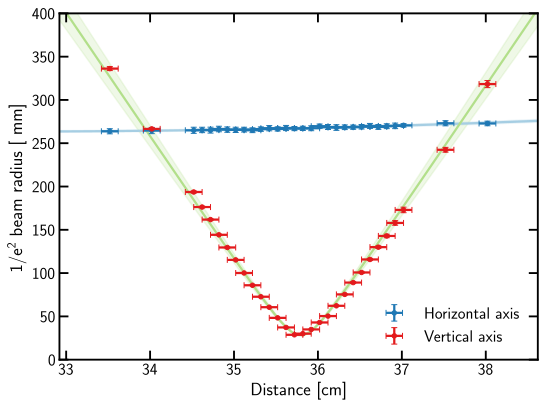
\includegraphics[keepaspectratio, width=4in]{experiment/odt_system/sheet_trap/sheet_trap_profile/sheet_profile.pdf}
	\caption[]{
		\label{fig:sheet_trap_profile}
		Beam profile of the sheet trap from which we fit to obtain the beam waists.
		For the vertical waist: $w = \SI{28.0+-1.0}{\um}$, $z_{0} = \SI{35.795+-0.009}{\cm}$, and $M^2 = \num{1.18+-0.04}$.
		For the horizontal waist: $w = \SI{263.5+-0.9}{\um}$, $z_{0} = \SI{32.3+-0.4}{\cm}$, and $M^2 = \num{1.0}$.
		Distances are measured from the end of the cage system assuming $\pm \SI{1}{\mm}$ uncertainty.}
\end{figure}
The horizontal trap frequency in the main ODT is increased with a circular ODT beam intersecting the sheet trap at a near vertical angle.
The measured beam profile of the vertical trap is shown in \cref{fig:vertical_trap_profile}.
\begin{figure}[!htbp]
	\centering
	\includegraphics[keepaspectratio, width=4in]{experiment/odt_system/vertical_trap/vertical_trap_profile/vertical_profile.pdf}
	\caption[]{
		\label{fig:vertical_trap_profile}
		Beam profile of the vertical trap from which we fit to obtain the beam waists.
		An assumed $\pm \SI{1}{\mm}$ uncertainty in the measured distance and $\pm \SI{5}{\um}$ uncertainty in the measured waist size.
		*** ADD WAIST VALUES ***}
\end{figure}
For each experiment, we routinely measure the trap oscillation frequencies for the sample of interest. 

We attempted to circularly polarized the vertical ODT so that it would minimize the differential shifts and enable cooling in to the ODT \cite{Ido2003.PRL.91.053001, Stellmer2013.PRA.87.013611} but we have not yet observed any improvement.
This lack of improvement is likely due to our $\SI{689}{\nm}$ laser system being too broad to take advantage of the reduced shifts.

\section{Making and Detecting Rydberg Atoms}

After creating an ultracold sample of strontium, a $\SI{320}{\nm}$ UV laser system is used to excite them to Rydberg states via the two-photon transition from the intermediate $\nSLJ{5s5p}{3}{P}{1}$ state.
Once the Rydberg atoms are created, they are detected by applying an electric field ramp that ionizes any Rydberg atoms created and directs them towards a micro-channel plate (MCP) detector for counting.
%The electric field system and charged particle detection will be detailed in Joe Whalen's upcoming Ph.D. thesis so they will only be briefly covered here. 

\subsection{$\SI{320}{\nm}$ UV Laser System}

Strontium Rydberg atoms are produced using a two-photon transition where a $\SI{689}{\nm}$ and a $\SI{320}{\nm}$ photon drives atoms from the $\nSLJ{5s^2}{1}{S}{0}$ ground state to either a $\nSLJ{5sns}{3}{S}{1}$ or $\nSLJ{5snd}{3}{D}{J}$ Rydberg state. 
Generation of the $\SI{320}{\nm}$ radiation starts with a tunable, narrow linewidth $\SI{1064}{\nm}$ seed laser that is amplified to about $\SI{7.5}{\watt}$ by a fiber amplifier\footnote{IPG Photonics YAR-15K-1064-LP-SF ytterbium fiber amplifier.}.
Two $\SI{1064}{\nm}$ seed lasers have been used for experiments: 
\begin{description}
	\item[Koheras Basik BMY10PztSPm, KOH2038] \hfill \\
		This laser is capable of continuously scanning multiple gigahertz with both temperature and piezo tuning so it's preferred for experiments requiring scans over large frequency ranges. 
		The narrowest $\SI{640}{\nm}$ lines observed with this seed are around $\SI{1}{\MHz}$, likely limited by the slow feedback bandwidth of the piezo element.
	\item[NP Photonics Rock RFLM-50-3-1064.53-1-S-0] \hfill \\
		The Rock's piezo feedback bandwidth is quite a bit better than the Koheras with the narrowest features observed being $\SI{\approx 300}{\kHz}$.
		Although the feedback bandwidth results with a narrow $\SI{640}{\nm}$ linewidth, temperature tuning is very slow which makes it difficult to continuously tune over large frequency ranges. 
\end{description}
The output of the fiber amplifier pumps a Lockheed Martin Aculight Argos Model 2400 CW optical parametric oscillator (OPO) modified with a sum frequency generation (SFG) stage. 
Similar to the system described in \cite{Mieth2014.OE.22.11182}, OPO-SFG is achieved by replacing the standard OPO crystal with a periodically poled, magnesium-oxide-doped lithium niobate crystal ({MgO:PPLN}) where the first section is designed for OPO and second section is designed for SFG.
The cavity dichroics were also replaced to facilitate generation of $\SI{640}{\nm}$ light.
The OPO section uses the $\lambda_{\text{P}} = \SI{1.064}{\um}$ pump to generate $\lambda_{\text{S}} = \SI{1.6}{\um}$ and $\lambda_{\text{I}} = \SI{3.2}{\um}$ light.
The SFG section then combines the $\lambda_{\text{S}} = \SI{1.6}{\um}$ with another $\lambda_{\text{P}} = \SI{1.064}{\um}$ to produce $\lambda_{\text{SFG}} = \SI{640}{\nm}$.

As mentioned in \cite{DeSalvo2015.PhD}, temperature tuning of the crystal is required for efficient $\SI{640}{\nm}$ generation but the Argos system was only designed for heating.
A workaround was developed where a water-cooling block is attached to the outside of the OPO cavity housing to lower the temperature enough to where the Argos' internal heater is capable of stabilizing the temperature (see \cref{fig:argos_opo}).
With this addition, we typically get about $\SIrange[range-phrase=-]{1}{1.5}{\watt}$ of $\SI{640}{\nm}$ light.
\begin{figure}[!htbp]
	\centering
	\includesvg[keepaspectratio, width=\textwidth, height=\textheight]{experiment/uv_system/argos_opo/argos_opo.svg}
	\caption[]{
		\label{fig:argos_opo}
		Picture of the Lockheed Martin Aculight Argos Model 2400 CW OPO with the custom water-cooling block attached to the cavity housing.
		The current tubing on the cooling block is too stiff to bend so the laser cover is left off.
		*** ADD OPTICAL LAYOUT IF I HAVE TIME ***}
\end{figure}

Stabilization of the $\SI{640}{\nm}$ laser frequency is accomplished with a transfer cavity lock \cite{Riedle1994.RSI.65.42, Bohlouli2006.RSI.77.093105, Leopold2016.APB.122.236} where the length of a tunable optical cavity is stabilized by locking a cavity resonance to the $\SI{689}{\nm}$ laser (which itself is stabilized to an atomic reference).
The $\SI{640}{\nm}$ laser is then stabilized by locking its frequency to a resonance of the cavity. 
Some of the details of our transfer cavity are documented in \cite{Zha2013.BS, DeSalvo2015.PhD}.
Briefly, our transfer cavity is constructed from an Invar body with the cavity mirrors attached to a piezoelectric (PZT) stack on each end. 
The PZT on one end is used to stabilize the cavity length to the $\SI{689}{\nm}$ laser while the other end provides a tunable offset cavity length that can be used to lock to different FSRs of the transfer cavity.
Pound-Drever-Hall (PDH) \cite{Drever1983.APB.31.97, Black2001.AJP.69.79} is used to lock the cavity length to the $\SI{689}{\nm}$ reference and to lock the $\SI{640}{\nm}$ to the cavity.
The optical layout at the transfer cavity is shown in \cref{fig:transfer_cavity}.
\begin{figure}[!htbp]
	\centering
	\includesvg[keepaspectratio, width=\textwidth, height=\textheight]{experiment/uv_system/transfer_cavity.svg}
	\caption[]{
		\label{fig:transfer_cavity}
		Simplified diagram of the transfer cavity setup for stabilizing the $\SI{640}{\nm}$ laser system. 
		The system is modified from the one presented in \cite{DeSalvo2015.PhD} with the addition of power control for reducing sensitivity to residual amplitude modulation (RAM).
		*** PUT FIBER EOM IN TO DIAGRAM ***}
\end{figure}
Tunability is achieved with a broadband fiber EOM (fEOM) between the OPO laser output and the transfer cavity which places tunable gigahertz sidebands on the $\SI{640}{\nm}$ light which can be locked to (e.g., see \cite{Gregory2015.NJP.17.055006}).
The PDH error signal is fed back to the $\SI{1064}{\nm}$ seed laser.
Although we have not done a full characterization of the linewidth of the $\SI{640}{\nm}$ laser, the narrowest Rydberg lines we have seen are about $\SI{150}{\kHz}$ (in $\SI{640}{\nm}$) with the Rock and can be considered an upper bound on the laser's short-term stability.
Longer-term stability isn't as good where drifts of $\SI{500}{\kHz}$ have been observed when scanning over the same Rydberg lines separated by a few days.
%With the recent acquisition of a ULE cavity (see \cref{ap:upgrades}), we plan to eliminate the transfer cavity in favor of locking the $\SI{640}{\nm}$ directly to the ULE cavity with a setup similar to the one presented in \cite{Gregory2015.NJP.17.055006}.

The $\SI{640}{\nm}$ output from the OPO is coupled into a commercial Toptica second-harmonic generation (SHG) pro system, which doubles the $\SI{640}{\nm}$ to $\SI{320}{\nm}$.
When well-tuned, the system is capable of outputting $\SI{> 500}{\milli\W}$ of power but it tends to degrade over time.
Our typical operating powers are closer to about $\SI{100}{\milli\W}$ and varies depending on the $n$ we are exciting.
\begin{figure}[!htbp]
	\centering
	\includesvg[keepaspectratio, width=\textwidth, height=\textheight]{experiment/uv_system/toptica_shg_pro/toptica_shg_pro-cavity.svg}
	\caption[]{
		\label{fig:toptica_shg_pro-cavity}
		Picture of the Toptica SHG pro bow tie doubling cavity. 
		The normally-sealed SHG cavity was opened up for realigning the $\SI{640}{\nm}$ to the SHG cavity.}
\end{figure}

\subsection{Electric Field System}

Due to the extreme ${n^\star}^{7}$ scaling of polarizability \cite{Gallagher1994.RydbergAtoms}, Rydberg atoms are extremely sensitive to electric fields. 
In-vacuum electric field plates were installed to mitigate stray electric fields at the location of the atoms as well as to provide the capability for trimming residual electric fields and for performing selective field ionization (SFI).
The electric field plate system, shown in \cref{fig:electric_field_system-CAD,fig:electric_field_system-real}, follows similar ones described in \cite{Millen2011.PhD, Low2012.JPB.45.113001} using a split-ring electrode geometry with four quadrant electrodes above and four quadrant electrodes below the atoms.
\begin{figure}[!htbp]
	\centering
	\includesvg[keepaspectratio, width=\textwidth, height=\textheight]{experiment/electric_field_system/electric_field_system-CAD.svg}
	\caption[]{
		\label{fig:electric_field_system-CAD}
		CAD renderings of the electric field plates with most of the supporting scaffold removed.
		Blue spheres represent the sapphire spacers used to isolate the high-voltage components from the grounded support structure.
		(Left) Top view of the eight electric field plates, Einzel lens, guiding plates, and MCP.
		The eleven \SI{10}{\kV} SHV feedthroughs are numbered clockwise.
		Red circles highlight the locations of the feedthroughs which are partially obstructed from view by the bottom scaffold plate.
		(Right) The electrodes are numbered corresponding to the feedthrough on the bottm flange.}
\end{figure}
\begin{figure}[!htbp]
	\centering
	\includesvg[keepaspectratio, width=\textwidth, height=\textheight]{experiment/electric_field_system/electric_field_system-real.svg}
	\caption[]{
		\label{fig:electric_field_system-real}
		(Left) Overview of the actual electric field system mounted on the bottom flange of main chamber. 
		Connections between the feedthroughs and the electric field plates are made with OFHC wires and insulated from the grounded supporting scaffold wtih ceramic fish spine beads. 
		Beryllium-copper in-line barrel connectors with two cross-screws attach the wires to the feedthroughs.
		(Right) Close up of the eight electric field plates, Einzel lens, and guiding plates.
		The sapphire spheres (red or clear) which isolate the high-voltage parts from the grounded scaffold structure are also visible.}
\end{figure}
The split-ring electrodes and in vacuum wires are made from oxygen-free high conductivity (OFHC) copper with stainless steel making up the supporting scaffold, Einzel lens, and guiding plates. 
Additional details can be found in \cite{Camargo2017.PhD}.

We currently have a (limited) ability to change how the electric field plates are ramped depending on whether want want to detect electrons or ions, and whether we want to perform state-resolved selective field ionization (SFI). 
Most of the work presented in this thesis involves detecting electrons and using the integrated SFI spectra (i.e., simply counting all the electrons). 
When taking data, we monitor the SFI spectra to make sure that the entire Rydberg signal is captured but the data analysis simply uses the total Rydberg electron counts. 
An example SFI spectrum is shown in \cref{fig:example_mcs_signal}. 

% Working at high-$n$, Soumya was able to trim electric fields to better than ** xxxx V/cm ** when taking spectra at $n=160$.
% We should be able to improve our electric field zeroing a bit more if we're more careful with biases on the SFI HV switches but extremely accurate switching would likely require going to a different design (** e.g. Tilman Pfau's box **).
% For now, the electric field system is sufficient for our purposes. 

\subsection{Charged Particle Detection}

One of the major aspects which separates this experiment from most other neutral atom experiments is the ability to detect charged particles. 
Some of the previous work with strontium Rydberg experiments was carried out in the Neutral apparatus but since it lacked the ability to detect charged particles, atom loss in absorption images was used instead \cite{DeSalvo2015.PRA.92.031403, DeSalvo2016.PRA.93.022709, Aman2016.PRA.93.043425}.
Our system was designed from the beginning to be able to detect charged particles have been incredibly sensitive and provides the ability to detect signals spanning several orders of magnitude \cite{Camargo2018.PRL.120.083401}.
%** Since Joe will be detailing the electric field ionization and detection system in his upcoming Ph.D. thesis, only the major details are included here for completeness. **

An overview of how the charged particle detection system works is shown in \cref{fig:charged_particle_detection}.
The following procedure outlines how electrons are detected but the system can be configured to detect ions instead.
After performing a Rydberg excitation on a sample, an electric field ramp is applied where the plates closer (further) from the MCP are ramped to positive (negative) high-voltage, ionizing any Rydberg atoms produced and directing the electrons towards the MCP. 
The length of the cables from the HV switch\footnote{Willamette High Voltage PHVSW-005.} to each of the feedthroughs are about the same length to keep the capacitances approximately equal.
\begin{figure}[!htbp]
	\centering
	\includesvg[keepaspectratio, width=\textwidth, height=\textheight]{experiment/mcp/charged_particle_detection.svg}
	\caption[]{
		\label{fig:charged_particle_detection}
		 Simplified diagram of how the charged particle detection system works when set up for counting electrons.}
\end{figure}
The high-voltage supplies for the electric field plate ramps are adjusted depending on the principal quantum number of the Rydberg state being excited.
Due to the cable capacitance, this also affects the ramp rate of the applied electric field but it doesn't significantly affect the integrated SFI spectrum which is the quantity of interest.

Charged particles are detected with an MCP\footnote{Photonis Advanced Performance Detector (APD) 2 miniTOF. It's important to note that we purchased the version with PEEK components so care must be taken when performing a bake-out.}.
For detecting electrons, the front plate is kept fixed at $\SI{200}{\V}$ while the back of the MCP is fixed at $\SI{2650}{\V}$.
The MCP is mounted to a $\SI{2.75}{\inch}$ flange with four HV feedthroughs with ceramic insulation.
\begin{figure}[!htbp]
	\centering
	\includesvg[keepaspectratio, width=\textwidth, height=\textheight]{experiment/mcp/mcp.svg}
	\caption[]{
		\label{fig:mcp}
		(Top left) The MCP mounted to a $\SI{2.75}{\inch}$ flange with high-voltage feedthroughs. 
		Connections are made using beryllium-copper inline barrel connectors with ceramic washers placed between the screws to keep the connections from touching each other and the main vacuum chamber.
		(Top right) The MCP in the main chamber.
		(Bottom) Mechanical drawing of the APD 2 miniTOF MCP provided by Photonis USA.
		*** MAKE BOTTOM FIGURE LARGER ***}
\end{figure}
Currently, the MCP's output is first connected to a preamplifier\footnote{Stanford Research Systems SR445.} which is then fed in to an RF amplifier\footnote{Mini-Circuits ZFL-500LN.} to remove DC offsets before going to the MCS\footnote{FAST ComTec GmbH MCA-3 P7882.}. 
An example Rydberg signal from the MCS is shown in \cref{fig:example_mcs_signal}.
\begin{figure}[!htbp]
	\centering
	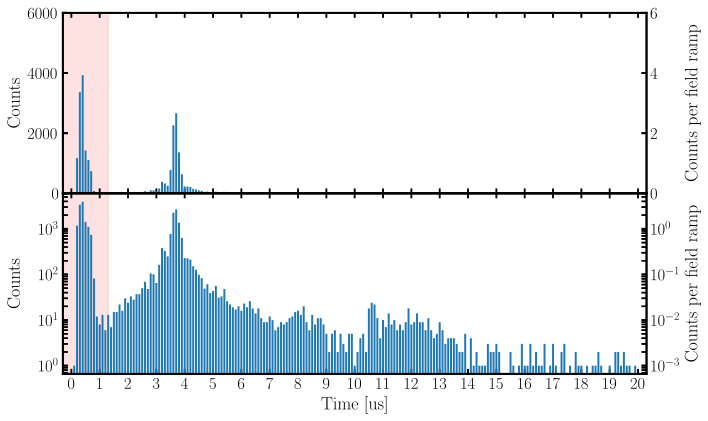
\includegraphics[keepaspectratio, width=\textwidth, height=\textheight]{experiment/mcp/example_mcs_signal/example_mcs_signal.pdf}
	\caption[]{
		\label{fig:example_mcs_signal}
		Example MCS signal from the $\nSLJf{5s38s}{3}{S}{1}{\flatfrac{11}{2}}$ Rydberg line in \Sr{87} for a single detuning in (top) linear scale and (bottom) log scale.
		There are $\num{200}$ $\SI{100}{\ns}$ bins with the electric field ramp starting at $t = \SI{0}{\ns}$.
		To increase signal, we perform multiple excitation-detection sequences and sum the resulting counts bin-by-bin. 
		Dividing by the total number of loops gives the counts per bin per loop ($\num{1000}$ loops were used in the data above).
		The MCS detects a large ``kick'' for first several bins (shaded region) so the data in those bins (shaded region) are dropped before proceeding with the analysis.}
\end{figure}

As seen in \cref{fig:mcp_saturation}, MCPs are known to ``saturate'' and become non-linear as the count rate increases.
This non-linearity is important to characterize to determine when the signal changes from the linear regime to the non-linear regime which requires the non-linearity to be taken in to account. 
\begin{figure}[!htbp]
	\centering
	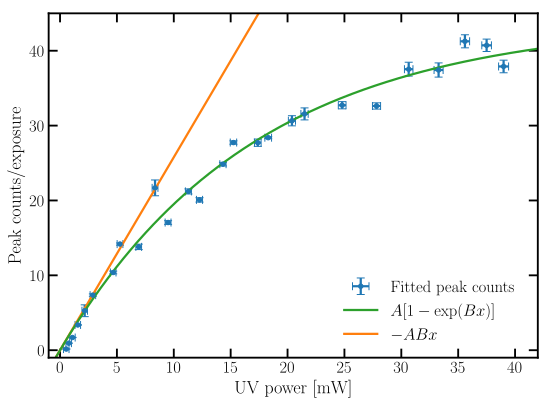
\includegraphics[keepaspectratio, width=\textwidth, height=\textheight]{experiment/mcp/mcp_saturation/20190327-Complete_data_set/mcp-counts_vs_uv_power.pdf}
	\caption[]{
		\label{fig:mcp_saturation}
		Peak integrated SFI spectrum per $\SI{10}{\us}$ exposure vs. UV excitation power exciting to the $\nSLJf{5s33s}{3}{S}{1}{\flatfrac{11}{2}}$ state of \Sr{87} in a $B_{x} \approx \SI{1.1}{\gauss}$ bias field (\SI{689}{\nm} power kept constant).
		The peak counts were obtained by fitting to the Zeeman-split spectra and extracting the height of the $m_{F} = \flatfrac{11}{2}$ line.
		Since $\num{1000}$ $\SI{10}{\us}$ exposures were used for each frequency point, the fitted peak counts was divided by $\num{1000}$ to obtain the counts per exposure.
		Fitting to the empirical model $A \qty[1 - \exp(B x)]$ results in the coefficients $A = \num{44.0+-1.7}$ and $B = \num{-0.059+-0.005}$.}
\end{figure}
Performing a fit to the empirical model
\begin{equation}
	y	=	A \qty[1 - \exp(B x)]
\end{equation}
determines the constants $A = \num{44.0+-1.7}$ and $B = \num{-0.059+-0.005}$, allowing for correction of undercounting in the non-linear regime. 
However, data are typically only recorded under conditions where teh departures from linearity are relatively small.